\documentclass[a4paper]{book}
\usepackage{makeidx}
\usepackage{natbib}
\usepackage{graphicx}
\usepackage{multicol}
\usepackage{float}
\usepackage{listings}
\usepackage{color}
\usepackage{ifthen}
\usepackage[table]{xcolor}
\usepackage{textcomp}
\usepackage{alltt}
\usepackage{ifpdf}
\ifpdf
\usepackage[pdftex,
            pagebackref=true,
            colorlinks=true,
            linkcolor=blue,
            unicode
           ]{hyperref}
\else
\usepackage[ps2pdf,
            pagebackref=true,
            colorlinks=true,
            linkcolor=blue,
            unicode
           ]{hyperref}
\usepackage{pspicture}
\fi
\usepackage[utf8]{inputenc}
\usepackage{mathptmx}
\usepackage[scaled=.90]{helvet}
\usepackage{courier}
\usepackage{sectsty}
\usepackage[titles]{tocloft}
\usepackage{doxygen}
\lstset{language=C++,inputencoding=utf8,basicstyle=\footnotesize,breaklines=true,breakatwhitespace=true,tabsize=8,numbers=left }
\makeindex
\setcounter{tocdepth}{3}
\renewcommand{\footrulewidth}{0.4pt}
\renewcommand{\familydefault}{\sfdefault}
\hfuzz=15pt
\setlength{\emergencystretch}{15pt}
\hbadness=750
\tolerance=750
\begin{document}
\hypersetup{pageanchor=false,citecolor=blue}
\begin{titlepage}
\vspace*{7cm}
\begin{center}
{\Large \-My \-Project }\\
\vspace*{1cm}
{\large \-Generated by Doxygen 1.7.6.1}\\
\vspace*{0.5cm}
{\small Thu Mar 27 2014 17:03:27}\\
\end{center}
\end{titlepage}
\clearemptydoublepage
\pagenumbering{roman}
\tableofcontents
\clearemptydoublepage
\pagenumbering{arabic}
\hypersetup{pageanchor=true,citecolor=blue}
\chapter{\-Namespace \-Index}
\section{\-Namespace \-List}
\-Here is a list of all documented namespaces with brief descriptions\-:\begin{DoxyCompactList}
\item\contentsline{section}{\hyperlink{namespacebezier}{bezier} }{\pageref{namespacebezier}}{}
\item\contentsline{section}{\hyperlink{namespacenozzle}{nozzle} }{\pageref{namespacenozzle}}{}
\item\contentsline{section}{\hyperlink{namespacepoint}{point} }{\pageref{namespacepoint}}{}
\end{DoxyCompactList}

\chapter{\-Class \-Index}
\section{\-Class \-Hierarchy}
\-This inheritance list is sorted roughly, but not completely, alphabetically\-:\begin{DoxyCompactList}
\item \contentsline{section}{bspline.\-Basis\-\_\-bspline}{\pageref{classbspline_1_1Basis__bspline}}{}
\item \contentsline{section}{geom\-\_\-2\-D.\-Bezier}{\pageref{classgeom__2D_1_1Bezier}}{}
\begin{DoxyCompactList}
\item \contentsline{section}{geom\-\_\-2\-D.\-Bezier\-\_\-\-Ar}{\pageref{classgeom__2D_1_1Bezier__Ar}}{}
\item \contentsline{section}{geom\-\_\-2\-D.\-Conv}{\pageref{classgeom__2D_1_1Conv}}{}
\item \contentsline{section}{geom\-\_\-2\-D.\-Div}{\pageref{classgeom__2D_1_1Div}}{}
\begin{DoxyCompactList}
\item \contentsline{section}{geom\-\_\-2\-D.\-B\-F\-\_\-div}{\pageref{classgeom__2D_1_1BF__div}}{}
\end{DoxyCompactList}
\end{DoxyCompactList}
\item \contentsline{section}{bezier.\-Bezier}{\pageref{classbezier_1_1Bezier}}{}
\begin{DoxyCompactList}
\item \contentsline{section}{nozzle.\-Conv}{\pageref{classnozzle_1_1Conv}}{}
\item \contentsline{section}{nozzle.\-Div}{\pageref{classnozzle_1_1Div}}{}
\begin{DoxyCompactList}
\item \contentsline{section}{nozzle.\-B\-F\-\_\-div}{\pageref{classnozzle_1_1BF__div}}{}
\end{DoxyCompactList}
\end{DoxyCompactList}
\item \contentsline{section}{cst.\-B\-F\-\_\-cst}{\pageref{classcst_1_1BF__cst}}{}
\item \contentsline{section}{bspline.\-Bspline}{\pageref{classbspline_1_1Bspline}}{}
\item \contentsline{section}{cst.\-Cst}{\pageref{classcst_1_1Cst}}{}
\item \contentsline{section}{bezier.\-Lagrange}{\pageref{classbezier_1_1Lagrange}}{}
\item \contentsline{section}{geom\-\_\-2\-D.\-Lagrange}{\pageref{classgeom__2D_1_1Lagrange}}{}
\item \contentsline{section}{nozzle.\-Nozzle}{\pageref{classnozzle_1_1Nozzle}}{}
\item \contentsline{section}{geom\-\_\-2\-D.\-Nozzle}{\pageref{classgeom__2D_1_1Nozzle}}{}
\item \contentsline{section}{geom\-\_\-2\-D.\-Plot}{\pageref{classgeom__2D_1_1Plot}}{}
\item \contentsline{section}{point.\-Point}{\pageref{classpoint_1_1Point}}{}
\item \contentsline{section}{geom\-\_\-2\-D.\-Point}{\pageref{classgeom__2D_1_1Point}}{}
\item \contentsline{section}{tut2.\-Uiuc\-Airfoil}{\pageref{classtut2_1_1UiucAirfoil}}{}
\end{DoxyCompactList}

\chapter{\-Class \-Index}
\section{\-Class \-List}
\-Here are the classes, structs, unions and interfaces with brief descriptions\-:\begin{DoxyCompactList}
\item\contentsline{section}{\hyperlink{classbspline_1_1Basis__bspline}{bspline.\-Basis\-\_\-bspline} }{\pageref{classbspline_1_1Basis__bspline}}{}
\item\contentsline{section}{\hyperlink{classgeom__2D_1_1Bezier}{geom\-\_\-2\-D.\-Bezier} }{\pageref{classgeom__2D_1_1Bezier}}{}
\item\contentsline{section}{\hyperlink{classbezier_1_1Bezier}{bezier.\-Bezier} }{\pageref{classbezier_1_1Bezier}}{}
\item\contentsline{section}{\hyperlink{classgeom__2D_1_1Bezier__Ar}{geom\-\_\-2\-D.\-Bezier\-\_\-\-Ar} }{\pageref{classgeom__2D_1_1Bezier__Ar}}{}
\item\contentsline{section}{\hyperlink{classcst_1_1BF__cst}{cst.\-B\-F\-\_\-cst} }{\pageref{classcst_1_1BF__cst}}{}
\item\contentsline{section}{\hyperlink{classnozzle_1_1BF__div}{nozzle.\-B\-F\-\_\-div} }{\pageref{classnozzle_1_1BF__div}}{}
\item\contentsline{section}{\hyperlink{classgeom__2D_1_1BF__div}{geom\-\_\-2\-D.\-B\-F\-\_\-div} }{\pageref{classgeom__2D_1_1BF__div}}{}
\item\contentsline{section}{\hyperlink{classbspline_1_1Bspline}{bspline.\-Bspline} }{\pageref{classbspline_1_1Bspline}}{}
\item\contentsline{section}{\hyperlink{classnozzle_1_1Conv}{nozzle.\-Conv} \\*\-N\-O\-O\-Z\-L\-E \-G\-E\-O }{\pageref{classnozzle_1_1Conv}}{}
\item\contentsline{section}{\hyperlink{classgeom__2D_1_1Conv}{geom\-\_\-2\-D.\-Conv} }{\pageref{classgeom__2D_1_1Conv}}{}
\item\contentsline{section}{\hyperlink{classcst_1_1Cst}{cst.\-Cst} }{\pageref{classcst_1_1Cst}}{}
\item\contentsline{section}{\hyperlink{classnozzle_1_1Div}{nozzle.\-Div} }{\pageref{classnozzle_1_1Div}}{}
\item\contentsline{section}{\hyperlink{classgeom__2D_1_1Div}{geom\-\_\-2\-D.\-Div} }{\pageref{classgeom__2D_1_1Div}}{}
\item\contentsline{section}{\hyperlink{classbezier_1_1Lagrange}{bezier.\-Lagrange} }{\pageref{classbezier_1_1Lagrange}}{}
\item\contentsline{section}{\hyperlink{classgeom__2D_1_1Lagrange}{geom\-\_\-2\-D.\-Lagrange} }{\pageref{classgeom__2D_1_1Lagrange}}{}
\item\contentsline{section}{\hyperlink{classnozzle_1_1Nozzle}{nozzle.\-Nozzle} }{\pageref{classnozzle_1_1Nozzle}}{}
\item\contentsline{section}{\hyperlink{classgeom__2D_1_1Nozzle}{geom\-\_\-2\-D.\-Nozzle} }{\pageref{classgeom__2D_1_1Nozzle}}{}
\item\contentsline{section}{\hyperlink{classgeom__2D_1_1Plot}{geom\-\_\-2\-D.\-Plot} }{\pageref{classgeom__2D_1_1Plot}}{}
\item\contentsline{section}{\hyperlink{classpoint_1_1Point}{point.\-Point} }{\pageref{classpoint_1_1Point}}{}
\item\contentsline{section}{\hyperlink{classgeom__2D_1_1Point}{geom\-\_\-2\-D.\-Point} }{\pageref{classgeom__2D_1_1Point}}{}
\item\contentsline{section}{\hyperlink{classtut2_1_1UiucAirfoil}{tut2.\-Uiuc\-Airfoil} }{\pageref{classtut2_1_1UiucAirfoil}}{}
\end{DoxyCompactList}

\chapter{\-Namespace \-Documentation}
\hypertarget{namespacebezier}{\section{bezier \-Namespace \-Reference}
\label{namespacebezier}\index{bezier@{bezier}}
}
\subsection*{\-Classes}
\begin{DoxyCompactItemize}
\item 
class \hyperlink{classbezier_1_1Lagrange}{\-Lagrange}
\item 
class \hyperlink{classbezier_1_1Bezier}{\-Bezier}
\end{DoxyCompactItemize}
\subsection*{\-Functions}
\begin{DoxyCompactItemize}
\item 
\hypertarget{namespacebezier_a584071379a6043563ba0b60ec8ead8eb}{def {\bfseries curvi\-\_\-abscissa}}\label{namespacebezier_a584071379a6043563ba0b60ec8ead8eb}

\end{DoxyCompactItemize}
\subsection*{\-Variables}
\begin{DoxyCompactItemize}
\item 
\hypertarget{namespacebezier_a35f64e1d41bd0a538b9a3a7640fffcc1}{tuple {\bfseries \-\_\-unzip} = lambdazipped\-:zip($\ast$zipped)}\label{namespacebezier_a35f64e1d41bd0a538b9a3a7640fffcc1}

\end{DoxyCompactItemize}


\subsection{\-Detailed \-Description}
\begin{DoxyVerb}@package zBlade
In this module it is implemented the class Bezier   
\end{DoxyVerb}
 
\hypertarget{namespacenozzle}{\section{nozzle \-Namespace \-Reference}
\label{namespacenozzle}\index{nozzle@{nozzle}}
}
\subsection*{\-Classes}
\begin{DoxyCompactItemize}
\item 
class \hyperlink{classnozzle_1_1Conv}{\-Conv}
\begin{DoxyCompactList}\small\item\em \-N\-O\-O\-Z\-L\-E \-G\-E\-O. \end{DoxyCompactList}\item 
class \hyperlink{classnozzle_1_1Div}{\-Div}
\item 
class \hyperlink{classnozzle_1_1Nozzle}{\-Nozzle}
\item 
class \hyperlink{classnozzle_1_1BF__div}{\-B\-F\-\_\-div}
\end{DoxyCompactItemize}
\subsection*{\-Variables}
\begin{DoxyCompactItemize}
\item 
\hypertarget{namespacenozzle_aaf7e494155ffd966b135ab1d9354f2b2}{string {\bfseries filename} = 'div.\-dat'}\label{namespacenozzle_aaf7e494155ffd966b135ab1d9354f2b2}

\item 
\hypertarget{namespacenozzle_a3db3842eb192143bc6255185f4eceedf}{tuple {\bfseries xy\-\_\-p} = pp.\-read\-\_\-xy\-\_\-p(filename)}\label{namespacenozzle_a3db3842eb192143bc6255185f4eceedf}

\item 
\hypertarget{namespacenozzle_a670c3cbec06a029072b73e7483eca284}{tuple {\bfseries fit} = \hyperlink{classnozzle_1_1BF__div}{\-B\-F\-\_\-div}(xy\-\_\-p, 5)}\label{namespacenozzle_a670c3cbec06a029072b73e7483eca284}

\item 
\hypertarget{namespacenozzle_a61477428c400085b4ff609d5385c8bee}{tuple {\bfseries \-Po} = fit.\-get\-\_\-cp()}\label{namespacenozzle_a61477428c400085b4ff609d5385c8bee}

\item 
\hypertarget{namespacenozzle_ae192cb9cc38b48c742ef3ed17add92f7}{tuple {\bfseries init\-\_\-guess} = \hyperlink{classbezier_1_1Bezier}{\-Bezier}(\-Po)}\label{namespacenozzle_ae192cb9cc38b48c742ef3ed17add92f7}

\item 
\hypertarget{namespacenozzle_afde5f5f5fca5b19f5bd1dfcfa36a3247}{tuple {\bfseries \-Ao} = fit.\-get\-\_\-\-A(\-Po)}\label{namespacenozzle_afde5f5f5fca5b19f5bd1dfcfa36a3247}

\item 
\hypertarget{namespacenozzle_a98f0fccf88dc387e14739aaad09c87cf}{tuple {\bfseries \-B} = fit.\-get\-\_\-bounds()}\label{namespacenozzle_a98f0fccf88dc387e14739aaad09c87cf}

\item 
\hypertarget{namespacenozzle_a0ccb978a357e0c50ba8877e672b9d1b9}{tuple {\bfseries \-A} = scipy.\-optimize.\-fmin\-\_\-slsqp(fit, \-Ao, bounds = \-B, iter = 1000)}\label{namespacenozzle_a0ccb978a357e0c50ba8877e672b9d1b9}

\item 
\hypertarget{namespacenozzle_a16247691e5be4b935e309b6d6062bbd2}{tuple {\bfseries \-P} = fit.\-get\-\_\-\-P(\-A)}\label{namespacenozzle_a16247691e5be4b935e309b6d6062bbd2}

\item 
\hypertarget{namespacenozzle_a5bc67755f1e5646f0b68c3ba88303578}{tuple {\bfseries fit\-\_\-curve} = \hyperlink{classbezier_1_1Bezier}{\-Bezier}(\-P)}\label{namespacenozzle_a5bc67755f1e5646f0b68c3ba88303578}

\item 
\hypertarget{namespacenozzle_a6baec50da90b88388370c11b7a4a1d12}{list {\bfseries err} = \mbox{[}0.\-765107371068, 0.\-381679555444, 0.\-371869452821, 0.\-332929094068, 0.\-307328456426\mbox{]}}\label{namespacenozzle_a6baec50da90b88388370c11b7a4a1d12}

\item 
\hypertarget{namespacenozzle_a12153924299e0f7ddc24c73c167da400}{list {\bfseries ncp} = \mbox{[}4, 5, 6, 7, 8\mbox{]}}\label{namespacenozzle_a12153924299e0f7ddc24c73c167da400}

\end{DoxyCompactItemize}


\subsection{\-Detailed \-Description}
\begin{DoxyVerb}@package zBlade
In this module it is implemented the a Geometrical modeller for a convergent-divergent Nozzle    
\end{DoxyVerb}
 
\hypertarget{namespacepoint}{\section{point \-Namespace \-Reference}
\label{namespacepoint}\index{point@{point}}
}
\subsection*{\-Classes}
\begin{DoxyCompactItemize}
\item 
class \hyperlink{classpoint_1_1Point}{\-Point}
\end{DoxyCompactItemize}


\subsection{\-Detailed \-Description}
\begin{DoxyVerb}@package zBlade
In this module it is implemented the class Point which represent 
the cartesian point    
\end{DoxyVerb}
 
\chapter{\-Class \-Documentation}
\hypertarget{classbspline_1_1Basis__bspline}{\section{bspline.\-Basis\-\_\-bspline \-Class \-Reference}
\label{classbspline_1_1Basis__bspline}\index{bspline.\-Basis\-\_\-bspline@{bspline.\-Basis\-\_\-bspline}}
}
\subsection*{\-Public \-Member \-Functions}
\begin{DoxyCompactItemize}
\item 
def \hyperlink{classbspline_1_1Basis__bspline_a5c48961d7e42050826953b47cb1cbd23}{\-\_\-\-\_\-init\-\_\-\-\_\-}
\item 
def \hyperlink{classbspline_1_1Basis__bspline_af18ccc4d68f6fd0662090d82dfb474a6}{\-\_\-\-\_\-call\-\_\-\-\_\-}
\item 
\hypertarget{classbspline_1_1Basis__bspline_a0db6a458c694d840c16e3016ede52dda}{def {\bfseries get\-\_\-span\-\_\-index}}\label{classbspline_1_1Basis__bspline_a0db6a458c694d840c16e3016ede52dda}

\end{DoxyCompactItemize}


\subsection{\-Constructor \& \-Destructor \-Documentation}
\hypertarget{classbspline_1_1Basis__bspline_a5c48961d7e42050826953b47cb1cbd23}{\index{bspline\-::\-Basis\-\_\-bspline@{bspline\-::\-Basis\-\_\-bspline}!\-\_\-\-\_\-init\-\_\-\-\_\-@{\-\_\-\-\_\-init\-\_\-\-\_\-}}
\index{\-\_\-\-\_\-init\-\_\-\-\_\-@{\-\_\-\-\_\-init\-\_\-\-\_\-}!bspline::Basis_bspline@{bspline\-::\-Basis\-\_\-bspline}}
\subsubsection[{\-\_\-\-\_\-init\-\_\-\-\_\-}]{\setlength{\rightskip}{0pt plus 5cm}def {\bf bspline.\-Basis\-\_\-bspline.\-\_\-\-\_\-init\-\_\-\-\_\-} (
\begin{DoxyParamCaption}
\item[{}]{self, }
\item[{}]{\-U, }
\item[{}]{p = {\ttfamily 0}}
\end{DoxyParamCaption}
)}}\label{classbspline_1_1Basis__bspline_a5c48961d7e42050826953b47cb1cbd23}
\begin{DoxyVerb}
construct Bspline basis function object

p == degree of the curve 
U == nonperiodic Knot vector  

identities:
m = len(U) - 1
n = m - p - 1

m+1 == length of the knot vector
n+1 == number basis function
\end{DoxyVerb}
 

\subsection{\-Member \-Function \-Documentation}
\hypertarget{classbspline_1_1Basis__bspline_af18ccc4d68f6fd0662090d82dfb474a6}{\index{bspline\-::\-Basis\-\_\-bspline@{bspline\-::\-Basis\-\_\-bspline}!\-\_\-\-\_\-call\-\_\-\-\_\-@{\-\_\-\-\_\-call\-\_\-\-\_\-}}
\index{\-\_\-\-\_\-call\-\_\-\-\_\-@{\-\_\-\-\_\-call\-\_\-\-\_\-}!bspline::Basis_bspline@{bspline\-::\-Basis\-\_\-bspline}}
\subsubsection[{\-\_\-\-\_\-call\-\_\-\-\_\-}]{\setlength{\rightskip}{0pt plus 5cm}def {\bf bspline.\-Basis\-\_\-bspline.\-\_\-\-\_\-call\-\_\-\-\_\-} (
\begin{DoxyParamCaption}
\item[{}]{self, }
\item[{}]{u}
\end{DoxyParamCaption}
)}}\label{classbspline_1_1Basis__bspline_af18ccc4d68f6fd0662090d82dfb474a6}
\begin{DoxyVerb}
this method compute the non vanishing basis function
Nurb book pag 70
\end{DoxyVerb}
 

\-The documentation for this class was generated from the following file\-:\begin{DoxyCompactItemize}
\item 
bspline.\-py\end{DoxyCompactItemize}

\hypertarget{classgeom__2D_1_1Bezier}{\section{geom\-\_\-2\-D.\-Bezier \-Class \-Reference}
\label{classgeom__2D_1_1Bezier}\index{geom\-\_\-2\-D.\-Bezier@{geom\-\_\-2\-D.\-Bezier}}
}
\-Inheritance diagram for geom\-\_\-2\-D.\-Bezier\-:\begin{figure}[H]
\begin{center}
\leavevmode
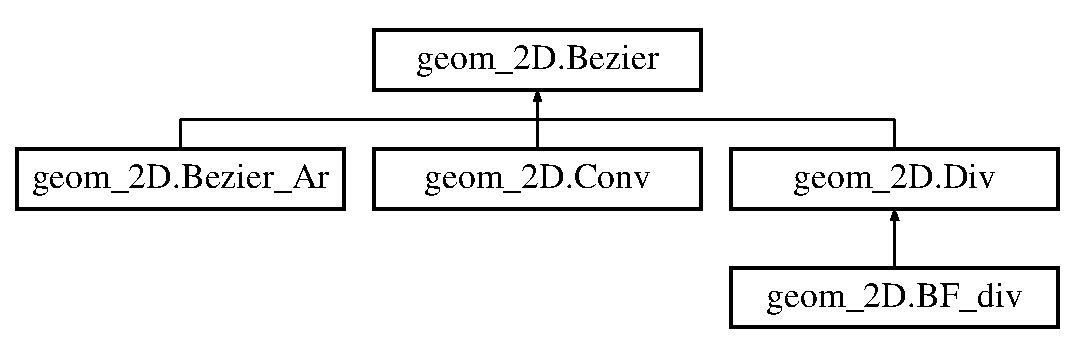
\includegraphics[height=3.000000cm]{classgeom__2D_1_1Bezier}
\end{center}
\end{figure}
\subsection*{\-Public \-Member \-Functions}
\begin{DoxyCompactItemize}
\item 
def \hyperlink{classgeom__2D_1_1Bezier_a57942b9390b8cb6e4245545661ee0e6b}{\-\_\-\-\_\-init\-\_\-\-\_\-}
\item 
\hypertarget{classgeom__2D_1_1Bezier_a5a5c7bd7306427c40aa976d6b5648909}{def {\bfseries sep}}\label{classgeom__2D_1_1Bezier_a5a5c7bd7306427c40aa976d6b5648909}

\item 
\hypertarget{classgeom__2D_1_1Bezier_a7627facb471c4d67d0f046460d37d38b}{def {\bfseries \-\_\-\-\_\-call\-\_\-\-\_\-}}\label{classgeom__2D_1_1Bezier_a7627facb471c4d67d0f046460d37d38b}

\item 
\hypertarget{classgeom__2D_1_1Bezier_a1c511284e0aa66764d016b5a2c7e9ab4}{def {\bfseries get\-\_\-cp}}\label{classgeom__2D_1_1Bezier_a1c511284e0aa66764d016b5a2c7e9ab4}

\item 
\hypertarget{classgeom__2D_1_1Bezier_a756cb59212797e9405dc6a4c1c2b07c7}{def {\bfseries get\-\_\-ncp}}\label{classgeom__2D_1_1Bezier_a756cb59212797e9405dc6a4c1c2b07c7}

\item 
\hypertarget{classgeom__2D_1_1Bezier_a659cf21f8e591685d99e82d3414c55a7}{def {\bfseries get\-\_\-x}}\label{classgeom__2D_1_1Bezier_a659cf21f8e591685d99e82d3414c55a7}

\item 
\hypertarget{classgeom__2D_1_1Bezier_af5420cd6be4a973b88e1d9401f8ff79b}{def {\bfseries get\-\_\-y}}\label{classgeom__2D_1_1Bezier_af5420cd6be4a973b88e1d9401f8ff79b}

\item 
\hypertarget{classgeom__2D_1_1Bezier_acaabdc283f18157a6525f2d47df24457}{def {\bfseries plot}}\label{classgeom__2D_1_1Bezier_acaabdc283f18157a6525f2d47df24457}

\end{DoxyCompactItemize}


\subsection{\-Constructor \& \-Destructor \-Documentation}
\hypertarget{classgeom__2D_1_1Bezier_a57942b9390b8cb6e4245545661ee0e6b}{\index{geom\-\_\-2\-D\-::\-Bezier@{geom\-\_\-2\-D\-::\-Bezier}!\-\_\-\-\_\-init\-\_\-\-\_\-@{\-\_\-\-\_\-init\-\_\-\-\_\-}}
\index{\-\_\-\-\_\-init\-\_\-\-\_\-@{\-\_\-\-\_\-init\-\_\-\-\_\-}!geom_2D::Bezier@{geom\-\_\-2\-D\-::\-Bezier}}
\subsubsection[{\-\_\-\-\_\-init\-\_\-\-\_\-}]{\setlength{\rightskip}{0pt plus 5cm}def {\bf geom\-\_\-2\-D.\-Bezier.\-\_\-\-\_\-init\-\_\-\-\_\-} (
\begin{DoxyParamCaption}
\item[{}]{self, }
\item[{}]{\-P, }
\item[{}]{discr = {\ttfamily 100}}
\end{DoxyParamCaption}
)}}\label{classgeom__2D_1_1Bezier_a57942b9390b8cb6e4245545661ee0e6b}
\begin{DoxyVerb}
construct bezier curve

P == list of control points
\end{DoxyVerb}
 

\-Reimplemented in \hyperlink{classgeom__2D_1_1BF__div_aaa1d864d0feadf18fb1848929ae2e6fd}{geom\-\_\-2\-D.\-B\-F\-\_\-div}.



\-The documentation for this class was generated from the following file\-:\begin{DoxyCompactItemize}
\item 
geom\-\_\-2\-D.\-py\end{DoxyCompactItemize}

\hypertarget{classbezier_1_1Bezier}{\section{bezier.\-Bezier \-Class \-Reference}
\label{classbezier_1_1Bezier}\index{bezier.\-Bezier@{bezier.\-Bezier}}
}
\-Inheritance diagram for bezier.\-Bezier\-:\begin{figure}[H]
\begin{center}
\leavevmode
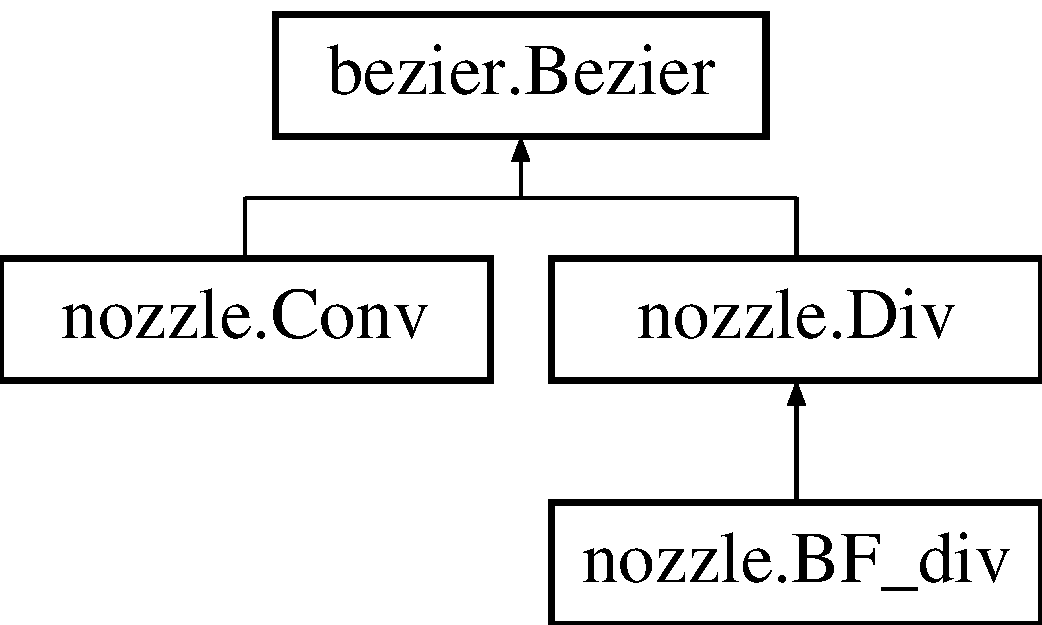
\includegraphics[height=3.000000cm]{classbezier_1_1Bezier}
\end{center}
\end{figure}
\subsection*{\-Public \-Member \-Functions}
\begin{DoxyCompactItemize}
\item 
def \hyperlink{classbezier_1_1Bezier_aa707e7f9dc64a98300877e9ce35e1cc3}{\-\_\-\-\_\-init\-\_\-\-\_\-}
\item 
\hypertarget{classbezier_1_1Bezier_ac23b42e2b53d6810f740099e28bee1cf}{def {\bfseries \-\_\-\-\_\-call\-\_\-\-\_\-}}\label{classbezier_1_1Bezier_ac23b42e2b53d6810f740099e28bee1cf}

\item 
\hypertarget{classbezier_1_1Bezier_aa366b876c53289e5fa811594b4923352}{def {\bfseries sep}}\label{classbezier_1_1Bezier_aa366b876c53289e5fa811594b4923352}

\item 
\hypertarget{classbezier_1_1Bezier_a755df32ec3b803a4a37a7b2674a7b8ef}{def {\bfseries get\-\_\-cp}}\label{classbezier_1_1Bezier_a755df32ec3b803a4a37a7b2674a7b8ef}

\item 
\hypertarget{classbezier_1_1Bezier_a5f731613c2f00dfbd6c97baf358fa53f}{def {\bfseries get\-\_\-ncp}}\label{classbezier_1_1Bezier_a5f731613c2f00dfbd6c97baf358fa53f}

\item 
\hypertarget{classbezier_1_1Bezier_aba655db92dafafdcaa193dd7fe98bb1e}{def {\bfseries get\-\_\-x}}\label{classbezier_1_1Bezier_aba655db92dafafdcaa193dd7fe98bb1e}

\item 
\hypertarget{classbezier_1_1Bezier_a6b9d505aa730b92dc227afbd05e08ddf}{def {\bfseries get\-\_\-y}}\label{classbezier_1_1Bezier_a6b9d505aa730b92dc227afbd05e08ddf}

\item 
\hypertarget{classbezier_1_1Bezier_ae6aa4066d6ba2c0432b388513a2998d4}{def {\bfseries get\-\_\-z}}\label{classbezier_1_1Bezier_ae6aa4066d6ba2c0432b388513a2998d4}

\item 
\hypertarget{classbezier_1_1Bezier_afa351a65d7f7bee24370ad50c2122a1f}{def {\bfseries get\-\_\-w}}\label{classbezier_1_1Bezier_afa351a65d7f7bee24370ad50c2122a1f}

\item 
\hypertarget{classbezier_1_1Bezier_a77482ccf5e7e4567e0f90b73a5bc8fd8}{def {\bfseries plot}}\label{classbezier_1_1Bezier_a77482ccf5e7e4567e0f90b73a5bc8fd8}

\end{DoxyCompactItemize}


\subsection{\-Constructor \& \-Destructor \-Documentation}
\hypertarget{classbezier_1_1Bezier_aa707e7f9dc64a98300877e9ce35e1cc3}{\index{bezier\-::\-Bezier@{bezier\-::\-Bezier}!\-\_\-\-\_\-init\-\_\-\-\_\-@{\-\_\-\-\_\-init\-\_\-\-\_\-}}
\index{\-\_\-\-\_\-init\-\_\-\-\_\-@{\-\_\-\-\_\-init\-\_\-\-\_\-}!bezier::Bezier@{bezier\-::\-Bezier}}
\subsubsection[{\-\_\-\-\_\-init\-\_\-\-\_\-}]{\setlength{\rightskip}{0pt plus 5cm}def {\bf bezier.\-Bezier.\-\_\-\-\_\-init\-\_\-\-\_\-} (
\begin{DoxyParamCaption}
\item[{}]{self, }
\item[{}]{\-P}
\end{DoxyParamCaption}
)}}\label{classbezier_1_1Bezier_aa707e7f9dc64a98300877e9ce35e1cc3}
\begin{DoxyVerb}
construct  rational bezier curve

P == list of control points
\end{DoxyVerb}
 

\-The documentation for this class was generated from the following file\-:\begin{DoxyCompactItemize}
\item 
bezier.\-py\end{DoxyCompactItemize}

\hypertarget{classgeom__2D_1_1Bezier__Ar}{\section{geom\-\_\-2\-D.\-Bezier\-\_\-\-Ar \-Class \-Reference}
\label{classgeom__2D_1_1Bezier__Ar}\index{geom\-\_\-2\-D.\-Bezier\-\_\-\-Ar@{geom\-\_\-2\-D.\-Bezier\-\_\-\-Ar}}
}
\-Inheritance diagram for geom\-\_\-2\-D.\-Bezier\-\_\-\-Ar\-:\begin{figure}[H]
\begin{center}
\leavevmode
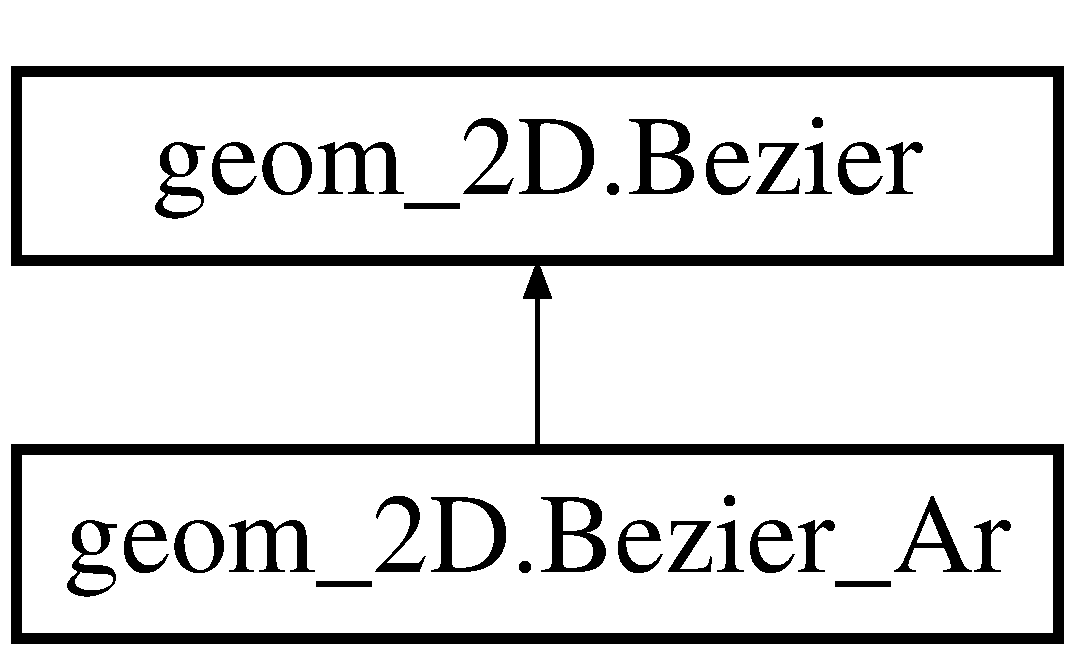
\includegraphics[height=2.000000cm]{classgeom__2D_1_1Bezier__Ar}
\end{center}
\end{figure}


\-The documentation for this class was generated from the following file\-:\begin{DoxyCompactItemize}
\item 
geom\-\_\-2\-D.\-py\end{DoxyCompactItemize}

\hypertarget{classcst_1_1BF__cst}{\section{cst.\-B\-F\-\_\-cst \-Class \-Reference}
\label{classcst_1_1BF__cst}\index{cst.\-B\-F\-\_\-cst@{cst.\-B\-F\-\_\-cst}}
}
\subsection*{\-Public \-Member \-Functions}
\begin{DoxyCompactItemize}
\item 
\hypertarget{classcst_1_1BF__cst_ab8b84510e4868e867cedae07c5e2b9e1}{def {\bfseries \-\_\-\-\_\-init\-\_\-\-\_\-}}\label{classcst_1_1BF__cst_ab8b84510e4868e867cedae07c5e2b9e1}

\item 
\hypertarget{classcst_1_1BF__cst_a8ca43a6e7a27cd85566ca627fdb91f73}{def {\bfseries \-\_\-\-\_\-call\-\_\-\-\_\-}}\label{classcst_1_1BF__cst_a8ca43a6e7a27cd85566ca627fdb91f73}

\end{DoxyCompactItemize}
\subsection*{\-Static \-Public \-Member \-Functions}
\begin{DoxyCompactItemize}
\item 
\hypertarget{classcst_1_1BF__cst_a524a2b94e57733cfae0b7aeb9ea0d94d}{def {\bfseries init\-\_\-cfc}}\label{classcst_1_1BF__cst_a524a2b94e57733cfae0b7aeb9ea0d94d}

\item 
\hypertarget{classcst_1_1BF__cst_ad18ba26bbf8cb290e7f4a12b290f46f4}{def {\bfseries init\-\_\-\-A}}\label{classcst_1_1BF__cst_ad18ba26bbf8cb290e7f4a12b290f46f4}

\item 
\hypertarget{classcst_1_1BF__cst_a55c2d1189db385093bd972cf80f40bb7}{def {\bfseries bound\-\_\-cfc}}\label{classcst_1_1BF__cst_a55c2d1189db385093bd972cf80f40bb7}

\item 
\hypertarget{classcst_1_1BF__cst_a41c0c602db45fa08f63f73d63203730c}{def {\bfseries bound\-\_\-\-A}}\label{classcst_1_1BF__cst_a41c0c602db45fa08f63f73d63203730c}

\end{DoxyCompactItemize}


\-The documentation for this class was generated from the following file\-:\begin{DoxyCompactItemize}
\item 
cst.\-py\end{DoxyCompactItemize}

\hypertarget{classnozzle_1_1BF__div}{\section{nozzle.\-B\-F\-\_\-div \-Class \-Reference}
\label{classnozzle_1_1BF__div}\index{nozzle.\-B\-F\-\_\-div@{nozzle.\-B\-F\-\_\-div}}
}
\-Inheritance diagram for nozzle.\-B\-F\-\_\-div\-:\begin{figure}[H]
\begin{center}
\leavevmode
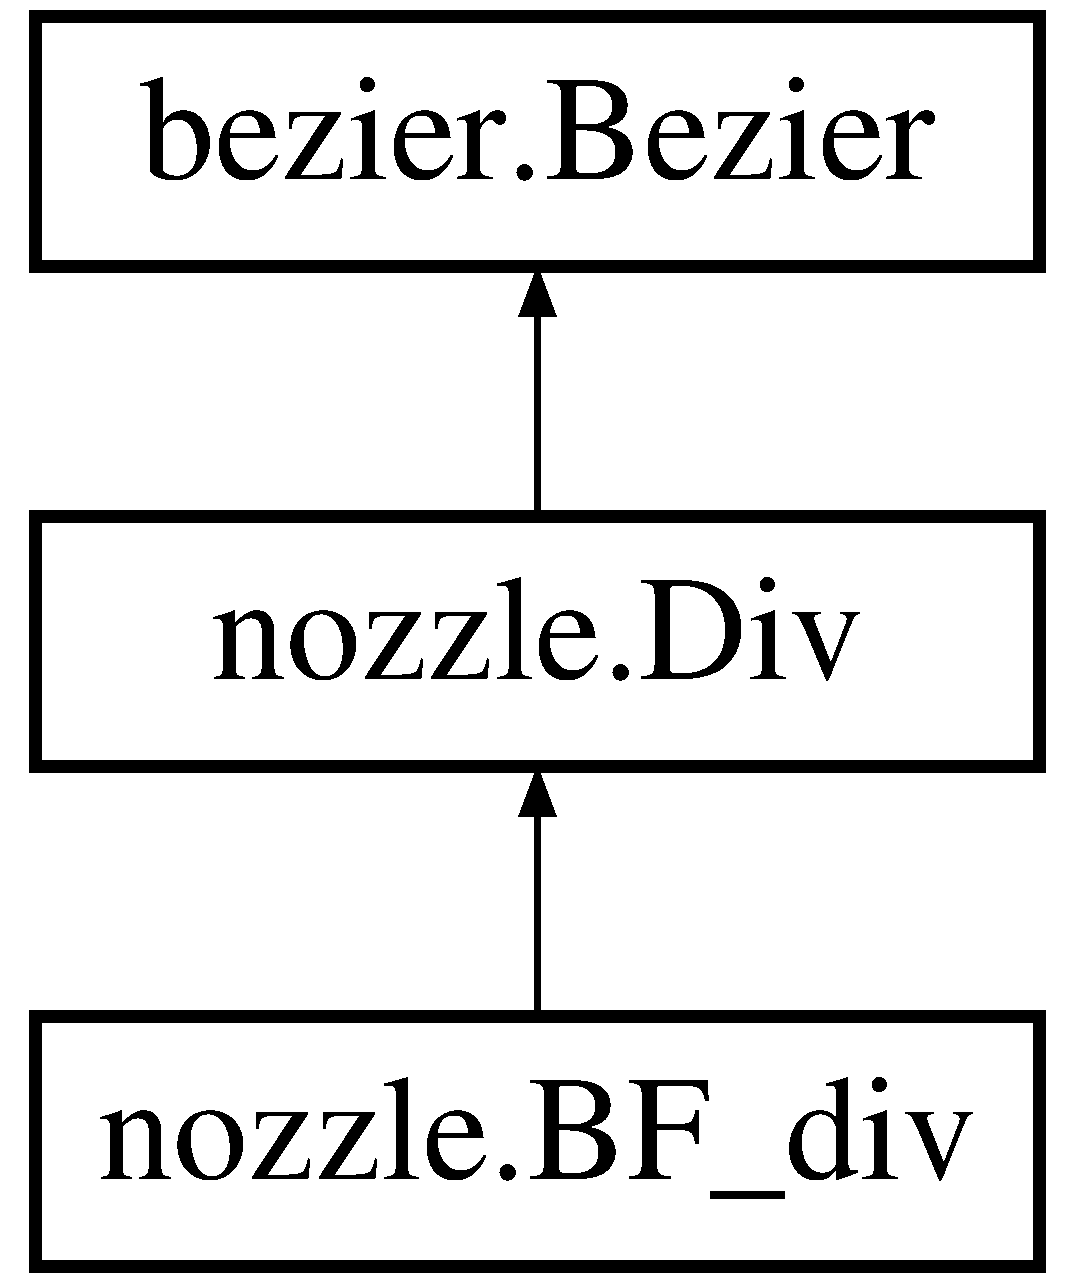
\includegraphics[height=3.000000cm]{classnozzle_1_1BF__div}
\end{center}
\end{figure}
\subsection*{\-Public \-Member \-Functions}
\begin{DoxyCompactItemize}
\item 
\hypertarget{classnozzle_1_1BF__div_a6587a3e9966faad931d46ab694eda13c}{def {\bfseries \-\_\-\-\_\-init\-\_\-\-\_\-}}\label{classnozzle_1_1BF__div_a6587a3e9966faad931d46ab694eda13c}

\item 
\hypertarget{classnozzle_1_1BF__div_af4c3cbda8c52d3ea68dc5097296e9799}{def {\bfseries \-\_\-\-\_\-call\-\_\-\-\_\-}}\label{classnozzle_1_1BF__div_af4c3cbda8c52d3ea68dc5097296e9799}

\item 
\hypertarget{classnozzle_1_1BF__div_ac5941d7080c648346029a7de5f392fd9}{def {\bfseries get\-\_\-\-P}}\label{classnozzle_1_1BF__div_ac5941d7080c648346029a7de5f392fd9}

\item 
\hypertarget{classnozzle_1_1BF__div_a78b7f95ae7ccdc18b5024f24925ef7dc}{def {\bfseries get\-\_\-\-A}}\label{classnozzle_1_1BF__div_a78b7f95ae7ccdc18b5024f24925ef7dc}

\item 
\hypertarget{classnozzle_1_1BF__div_a3907b91e2e0035b7449ec46d82d3fec5}{def {\bfseries get\-\_\-bounds}}\label{classnozzle_1_1BF__div_a3907b91e2e0035b7449ec46d82d3fec5}

\end{DoxyCompactItemize}


\-The documentation for this class was generated from the following file\-:\begin{DoxyCompactItemize}
\item 
nozzle.\-py\end{DoxyCompactItemize}

\hypertarget{classgeom__2D_1_1BF__div}{\section{geom\-\_\-2\-D.\-B\-F\-\_\-div \-Class \-Reference}
\label{classgeom__2D_1_1BF__div}\index{geom\-\_\-2\-D.\-B\-F\-\_\-div@{geom\-\_\-2\-D.\-B\-F\-\_\-div}}
}
\-Inheritance diagram for geom\-\_\-2\-D.\-B\-F\-\_\-div\-:\begin{figure}[H]
\begin{center}
\leavevmode
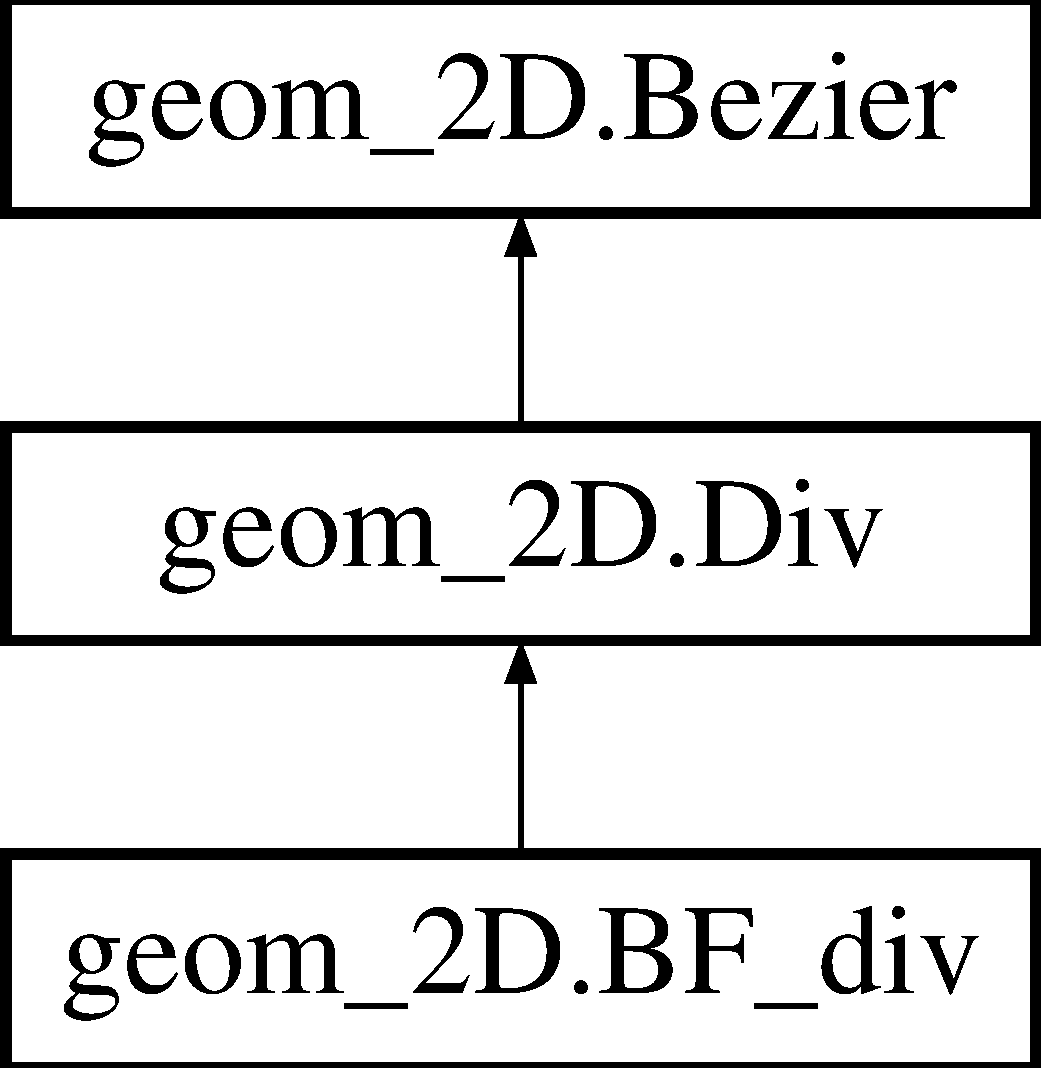
\includegraphics[height=3.000000cm]{classgeom__2D_1_1BF__div}
\end{center}
\end{figure}
\subsection*{\-Public \-Member \-Functions}
\begin{DoxyCompactItemize}
\item 
def \hyperlink{classgeom__2D_1_1BF__div_aaa1d864d0feadf18fb1848929ae2e6fd}{\-\_\-\-\_\-init\-\_\-\-\_\-}
\item 
\hypertarget{classgeom__2D_1_1BF__div_a17f5026ec01f75aff003d08f236c08c2}{def {\bfseries \-\_\-\-\_\-call\-\_\-\-\_\-}}\label{classgeom__2D_1_1BF__div_a17f5026ec01f75aff003d08f236c08c2}

\item 
\hypertarget{classgeom__2D_1_1BF__div_ac7542314ee6bb318cd8ad621d2ab2e72}{def {\bfseries get\-\_\-\-P}}\label{classgeom__2D_1_1BF__div_ac7542314ee6bb318cd8ad621d2ab2e72}

\item 
\hypertarget{classgeom__2D_1_1BF__div_a8cb77aa5cc80d09442e7026c43fb83eb}{def {\bfseries get\-\_\-\-A}}\label{classgeom__2D_1_1BF__div_a8cb77aa5cc80d09442e7026c43fb83eb}

\item 
\hypertarget{classgeom__2D_1_1BF__div_a9430bb46fcb27cd2caaf01710a09e944}{def {\bfseries get\-\_\-bounds}}\label{classgeom__2D_1_1BF__div_a9430bb46fcb27cd2caaf01710a09e944}

\end{DoxyCompactItemize}


\subsection{\-Constructor \& \-Destructor \-Documentation}
\hypertarget{classgeom__2D_1_1BF__div_aaa1d864d0feadf18fb1848929ae2e6fd}{\index{geom\-\_\-2\-D\-::\-B\-F\-\_\-div@{geom\-\_\-2\-D\-::\-B\-F\-\_\-div}!\-\_\-\-\_\-init\-\_\-\-\_\-@{\-\_\-\-\_\-init\-\_\-\-\_\-}}
\index{\-\_\-\-\_\-init\-\_\-\-\_\-@{\-\_\-\-\_\-init\-\_\-\-\_\-}!geom_2D::BF_div@{geom\-\_\-2\-D\-::\-B\-F\-\_\-div}}
\subsubsection[{\-\_\-\-\_\-init\-\_\-\-\_\-}]{\setlength{\rightskip}{0pt plus 5cm}def {\bf geom\-\_\-2\-D.\-B\-F\-\_\-div.\-\_\-\-\_\-init\-\_\-\-\_\-} (
\begin{DoxyParamCaption}
\item[{}]{self, }
\item[{}]{\-P, }
\item[{}]{discr = {\ttfamily 4}}
\end{DoxyParamCaption}
)}}\label{classgeom__2D_1_1BF__div_aaa1d864d0feadf18fb1848929ae2e6fd}
\begin{DoxyVerb}
construct bezier curve

P == list of control points
\end{DoxyVerb}
 

\-Reimplemented from \hyperlink{classgeom__2D_1_1Bezier_a57942b9390b8cb6e4245545661ee0e6b}{geom\-\_\-2\-D.\-Bezier}.



\-The documentation for this class was generated from the following file\-:\begin{DoxyCompactItemize}
\item 
geom\-\_\-2\-D.\-py\end{DoxyCompactItemize}

\hypertarget{classbspline_1_1Bspline}{\section{bspline.\-Bspline \-Class \-Reference}
\label{classbspline_1_1Bspline}\index{bspline.\-Bspline@{bspline.\-Bspline}}
}
\subsection*{\-Public \-Member \-Functions}
\begin{DoxyCompactItemize}
\item 
def \hyperlink{classbspline_1_1Bspline_a6ff60f8423946ec65f8e74ea4790c177}{\-\_\-\-\_\-init\-\_\-\-\_\-}
\item 
\hypertarget{classbspline_1_1Bspline_a791969b1414f2f8e1c03de6af94ad2a3}{def {\bfseries get\-\_\-\-U}}\label{classbspline_1_1Bspline_a791969b1414f2f8e1c03de6af94ad2a3}

\end{DoxyCompactItemize}


\subsection{\-Detailed \-Description}
\begin{DoxyVerb}
This class implement a rational Bspline with a nonperiodic uniform
knot vectors (definition at pag 66-67 of Nurbs book). 
\end{DoxyVerb}
 

\subsection{\-Constructor \& \-Destructor \-Documentation}
\hypertarget{classbspline_1_1Bspline_a6ff60f8423946ec65f8e74ea4790c177}{\index{bspline\-::\-Bspline@{bspline\-::\-Bspline}!\-\_\-\-\_\-init\-\_\-\-\_\-@{\-\_\-\-\_\-init\-\_\-\-\_\-}}
\index{\-\_\-\-\_\-init\-\_\-\-\_\-@{\-\_\-\-\_\-init\-\_\-\-\_\-}!bspline::Bspline@{bspline\-::\-Bspline}}
\subsubsection[{\-\_\-\-\_\-init\-\_\-\-\_\-}]{\setlength{\rightskip}{0pt plus 5cm}def {\bf bspline.\-Bspline.\-\_\-\-\_\-init\-\_\-\-\_\-} (
\begin{DoxyParamCaption}
\item[{}]{self, }
\item[{}]{\-P, }
\item[{}]{p = {\ttfamily 2}, }
\item[{}]{a = {\ttfamily 0}, }
\item[{}]{b = {\ttfamily 1}}
\end{DoxyParamCaption}
)}}\label{classbspline_1_1Bspline_a6ff60f8423946ec65f8e74ea4790c177}
\begin{DoxyVerb}
Constructor 
input:
p == degree of the curve 
P == list of control point   
a == lower bound of the interval for the knot vector domain
b == upper bound of the interval for the knot vector domain


identities:
n+1 = len(P) number of cont. Point namely number of basis function
m+1 = len(U) length of the knot vector
m = n + p + 1
\end{DoxyVerb}
 

\-The documentation for this class was generated from the following file\-:\begin{DoxyCompactItemize}
\item 
bspline.\-py\end{DoxyCompactItemize}

\hypertarget{classnozzle_1_1Conv}{\section{nozzle.\-Conv \-Class \-Reference}
\label{classnozzle_1_1Conv}\index{nozzle.\-Conv@{nozzle.\-Conv}}
}


\-N\-O\-O\-Z\-L\-E \-G\-E\-O.  


\-Inheritance diagram for nozzle.\-Conv\-:\begin{figure}[H]
\begin{center}
\leavevmode
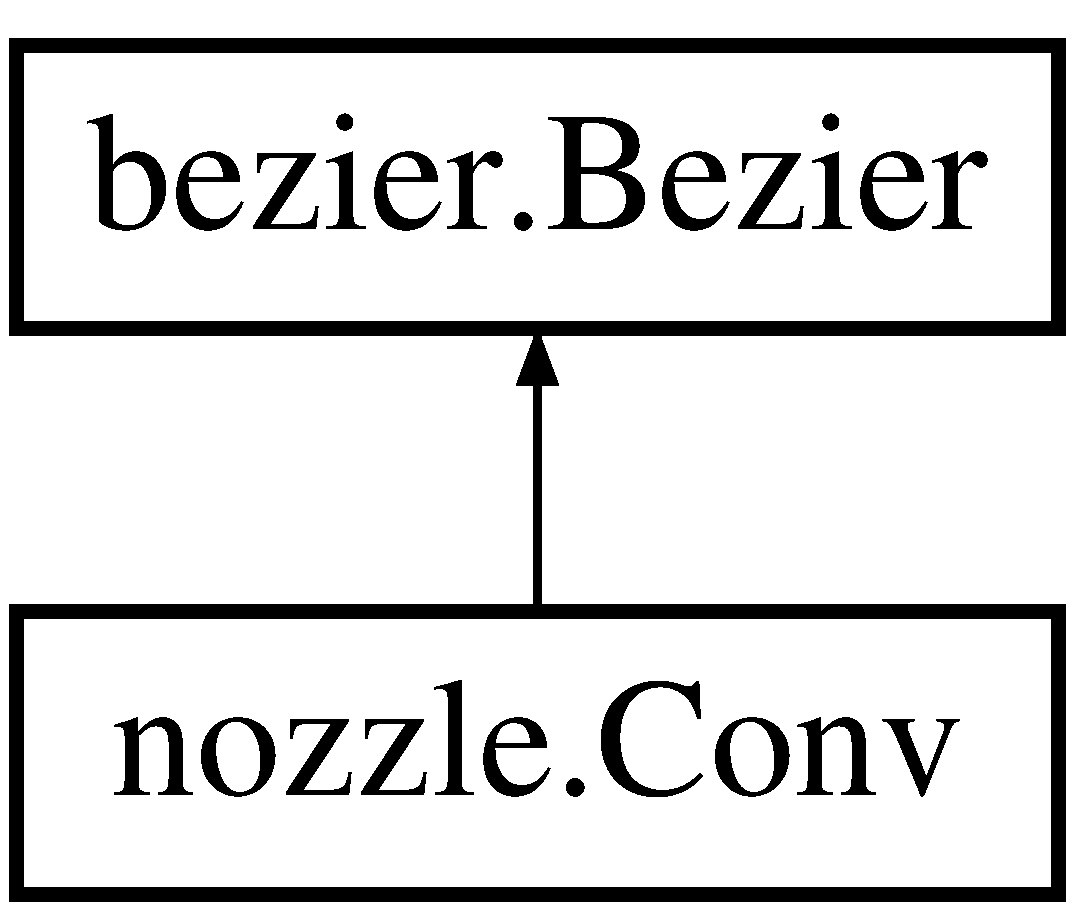
\includegraphics[height=2.000000cm]{classnozzle_1_1Conv}
\end{center}
\end{figure}
\subsection*{\-Public \-Member \-Functions}
\begin{DoxyCompactItemize}
\item 
\hypertarget{classnozzle_1_1Conv_a5bca41eac14d44bc02a31a8c66e05f95}{def {\bfseries \-\_\-\-\_\-init\-\_\-\-\_\-}}\label{classnozzle_1_1Conv_a5bca41eac14d44bc02a31a8c66e05f95}

\end{DoxyCompactItemize}


\subsection{\-Detailed \-Description}
\-N\-O\-O\-Z\-L\-E \-G\-E\-O. 

\-M\-O\-D\-E\-L\-E\-R \#\#\#\#\#\#\#\#\#\#\#\#\#\#\#\#\#\#\#\#\#\#\#\#\#\#\#\#\#\#\#\#\#\#\#\#\#\#\#\#\#\#\#\#\#\#\#\#\#\#\#\#\#\#\#\#\#\#\#\#\#\#\# 

\-The documentation for this class was generated from the following file\-:\begin{DoxyCompactItemize}
\item 
nozzle.\-py\end{DoxyCompactItemize}

\hypertarget{classgeom__2D_1_1Conv}{\section{geom\-\_\-2\-D.\-Conv \-Class \-Reference}
\label{classgeom__2D_1_1Conv}\index{geom\-\_\-2\-D.\-Conv@{geom\-\_\-2\-D.\-Conv}}
}
\-Inheritance diagram for geom\-\_\-2\-D.\-Conv\-:\begin{figure}[H]
\begin{center}
\leavevmode
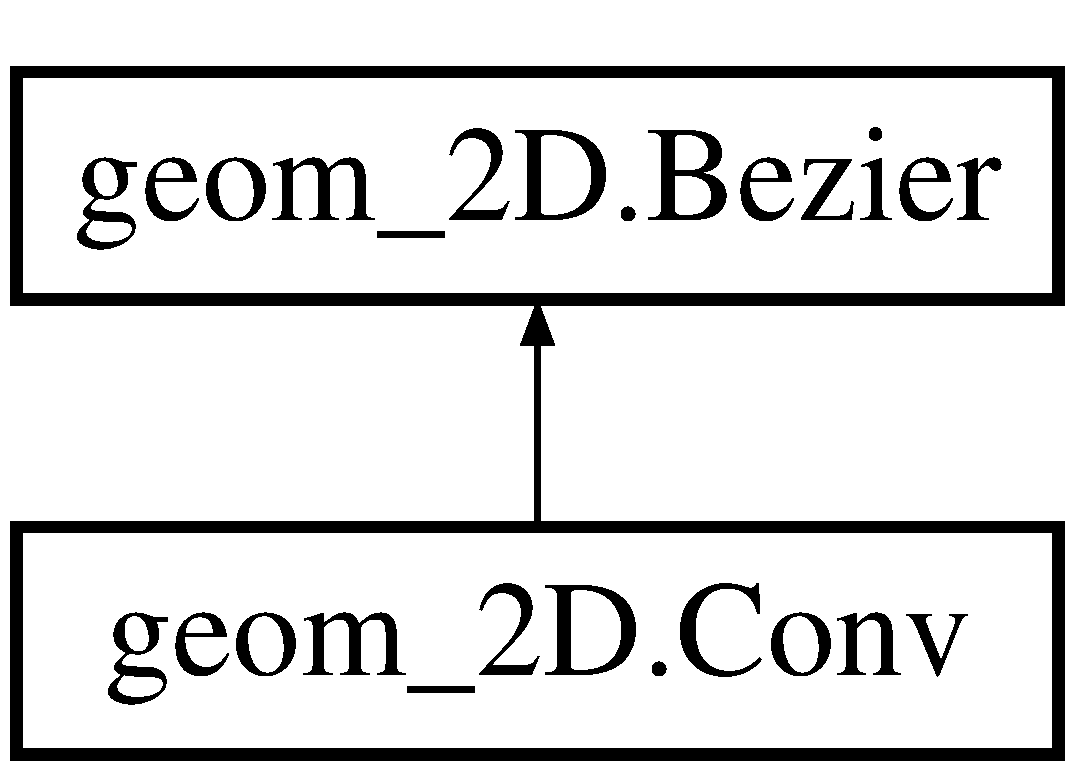
\includegraphics[height=2.000000cm]{classgeom__2D_1_1Conv}
\end{center}
\end{figure}
\subsection*{\-Public \-Member \-Functions}
\begin{DoxyCompactItemize}
\item 
\hypertarget{classgeom__2D_1_1Conv_aa021157b9808ed9ac5dbe72693697db4}{def {\bfseries \-\_\-\-\_\-init\-\_\-\-\_\-}}\label{classgeom__2D_1_1Conv_aa021157b9808ed9ac5dbe72693697db4}

\end{DoxyCompactItemize}


\-The documentation for this class was generated from the following file\-:\begin{DoxyCompactItemize}
\item 
geom\-\_\-2\-D.\-py\end{DoxyCompactItemize}

\hypertarget{classcst_1_1Cst}{\section{cst.\-Cst \-Class \-Reference}
\label{classcst_1_1Cst}\index{cst.\-Cst@{cst.\-Cst}}
}
\subsection*{\-Public \-Member \-Functions}
\begin{DoxyCompactItemize}
\item 
\hypertarget{classcst_1_1Cst_aa2b939a4963ef6e945b4162881e9e921}{def {\bfseries \-\_\-\-\_\-init\-\_\-\-\_\-}}\label{classcst_1_1Cst_aa2b939a4963ef6e945b4162881e9e921}

\item 
\hypertarget{classcst_1_1Cst_ad90496107430d6d6b517b31269398898}{def {\bfseries \-\_\-\-\_\-call\-\_\-\-\_\-}}\label{classcst_1_1Cst_ad90496107430d6d6b517b31269398898}

\end{DoxyCompactItemize}


\-The documentation for this class was generated from the following file\-:\begin{DoxyCompactItemize}
\item 
cst.\-py\end{DoxyCompactItemize}

\hypertarget{classnozzle_1_1Div}{\section{nozzle.\-Div \-Class \-Reference}
\label{classnozzle_1_1Div}\index{nozzle.\-Div@{nozzle.\-Div}}
}
\-Inheritance diagram for nozzle.\-Div\-:\begin{figure}[H]
\begin{center}
\leavevmode
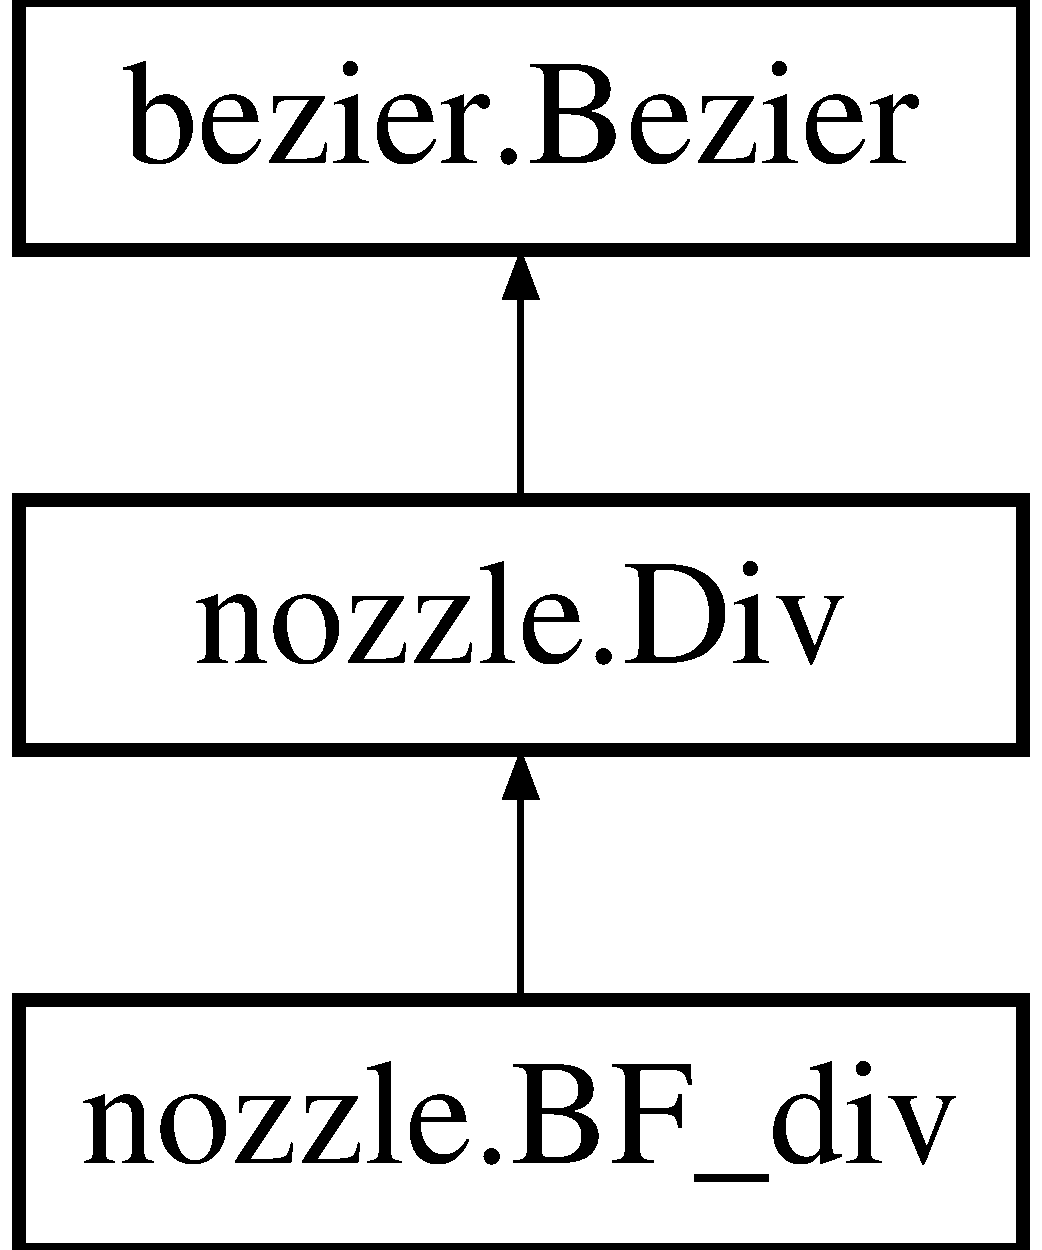
\includegraphics[height=3.000000cm]{classnozzle_1_1Div}
\end{center}
\end{figure}
\subsection*{\-Public \-Member \-Functions}
\begin{DoxyCompactItemize}
\item 
\hypertarget{classnozzle_1_1Div_a891afdf97cfb67f01f318f77c700d576}{def {\bfseries \-\_\-\-\_\-init\-\_\-\-\_\-}}\label{classnozzle_1_1Div_a891afdf97cfb67f01f318f77c700d576}

\end{DoxyCompactItemize}


\-The documentation for this class was generated from the following file\-:\begin{DoxyCompactItemize}
\item 
nozzle.\-py\end{DoxyCompactItemize}

\hypertarget{classgeom__2D_1_1Div}{\section{geom\-\_\-2\-D.\-Div \-Class \-Reference}
\label{classgeom__2D_1_1Div}\index{geom\-\_\-2\-D.\-Div@{geom\-\_\-2\-D.\-Div}}
}
\-Inheritance diagram for geom\-\_\-2\-D.\-Div\-:\begin{figure}[H]
\begin{center}
\leavevmode
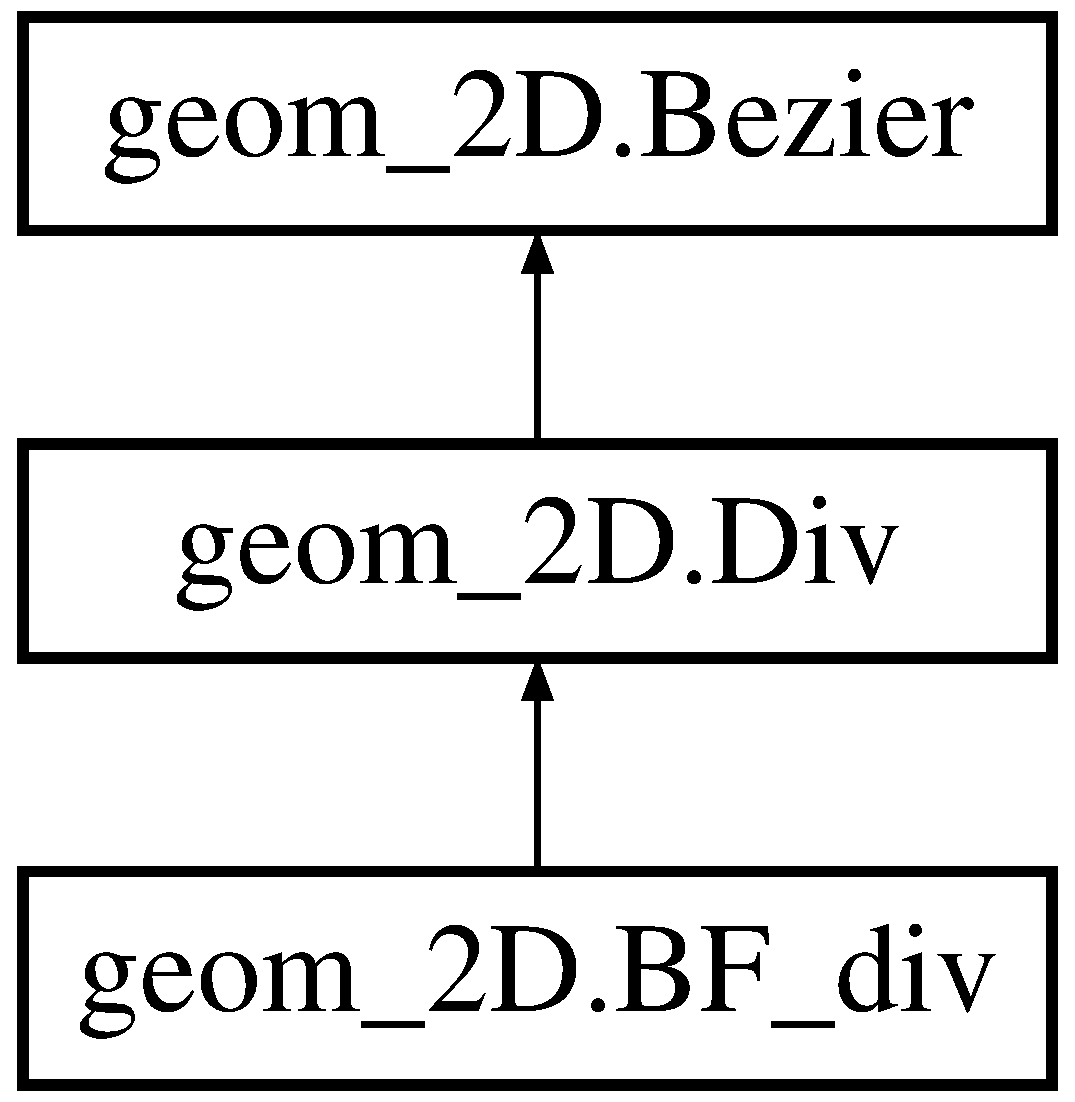
\includegraphics[height=3.000000cm]{classgeom__2D_1_1Div}
\end{center}
\end{figure}
\subsection*{\-Public \-Member \-Functions}
\begin{DoxyCompactItemize}
\item 
\hypertarget{classgeom__2D_1_1Div_aa765d65f15eebda96d87be39d9570808}{def {\bfseries \-\_\-\-\_\-init\-\_\-\-\_\-}}\label{classgeom__2D_1_1Div_aa765d65f15eebda96d87be39d9570808}

\end{DoxyCompactItemize}


\-The documentation for this class was generated from the following file\-:\begin{DoxyCompactItemize}
\item 
geom\-\_\-2\-D.\-py\end{DoxyCompactItemize}

\hypertarget{classbezier_1_1Lagrange}{\section{bezier.\-Lagrange \-Class \-Reference}
\label{classbezier_1_1Lagrange}\index{bezier.\-Lagrange@{bezier.\-Lagrange}}
}
\subsection*{\-Public \-Member \-Functions}
\begin{DoxyCompactItemize}
\item 
def \hyperlink{classbezier_1_1Lagrange_a99ddbd500e164e036507cb2d68c18969}{\-\_\-\-\_\-init\-\_\-\-\_\-}
\item 
def \hyperlink{classbezier_1_1Lagrange_ab27c64919a3450dc17d8d1d7f6a609a5}{\-\_\-\-\_\-call\-\_\-\-\_\-}
\end{DoxyCompactItemize}
\subsection*{\-Public \-Attributes}
\begin{DoxyCompactItemize}
\item 
\hypertarget{classbezier_1_1Lagrange_ac733ebcbd52d593fd7263cc70334181f}{{\bfseries \-Y}}\label{classbezier_1_1Lagrange_ac733ebcbd52d593fd7263cc70334181f}

\item 
\hypertarget{classbezier_1_1Lagrange_a8a9a9ec1c41f5645012b2bf2d52053ce}{{\bfseries t}}\label{classbezier_1_1Lagrange_a8a9a9ec1c41f5645012b2bf2d52053ce}

\end{DoxyCompactItemize}


\subsection{\-Constructor \& \-Destructor \-Documentation}
\hypertarget{classbezier_1_1Lagrange_a99ddbd500e164e036507cb2d68c18969}{\index{bezier\-::\-Lagrange@{bezier\-::\-Lagrange}!\-\_\-\-\_\-init\-\_\-\-\_\-@{\-\_\-\-\_\-init\-\_\-\-\_\-}}
\index{\-\_\-\-\_\-init\-\_\-\-\_\-@{\-\_\-\-\_\-init\-\_\-\-\_\-}!bezier::Lagrange@{bezier\-::\-Lagrange}}
\subsubsection[{\-\_\-\-\_\-init\-\_\-\-\_\-}]{\setlength{\rightskip}{0pt plus 5cm}def {\bf bezier.\-Lagrange.\-\_\-\-\_\-init\-\_\-\-\_\-} (
\begin{DoxyParamCaption}
\item[{}]{self, }
\item[{}]{\-P, }
\item[{}]{t}
\end{DoxyParamCaption}
)}}\label{classbezier_1_1Lagrange_a99ddbd500e164e036507cb2d68c18969}
\begin{DoxyVerb}
construct Lagrange curve function

P == list of control points
t == list of time points
len(P) == len(t)
\end{DoxyVerb}
 

\subsection{\-Member \-Function \-Documentation}
\hypertarget{classbezier_1_1Lagrange_ab27c64919a3450dc17d8d1d7f6a609a5}{\index{bezier\-::\-Lagrange@{bezier\-::\-Lagrange}!\-\_\-\-\_\-call\-\_\-\-\_\-@{\-\_\-\-\_\-call\-\_\-\-\_\-}}
\index{\-\_\-\-\_\-call\-\_\-\-\_\-@{\-\_\-\-\_\-call\-\_\-\-\_\-}!bezier::Lagrange@{bezier\-::\-Lagrange}}
\subsubsection[{\-\_\-\-\_\-call\-\_\-\-\_\-}]{\setlength{\rightskip}{0pt plus 5cm}def {\bf bezier.\-Lagrange.\-\_\-\-\_\-call\-\_\-\-\_\-} (
\begin{DoxyParamCaption}
\item[{}]{self, }
\item[{}]{t\-\_\-}
\end{DoxyParamCaption}
)}}\label{classbezier_1_1Lagrange_ab27c64919a3450dc17d8d1d7f6a609a5}
\begin{DoxyVerb}
return point on Langrange function at t_
\end{DoxyVerb}
 

\-The documentation for this class was generated from the following file\-:\begin{DoxyCompactItemize}
\item 
bezier.\-py\end{DoxyCompactItemize}

\hypertarget{classgeom__2D_1_1Lagrange}{\section{geom\-\_\-2\-D.\-Lagrange \-Class \-Reference}
\label{classgeom__2D_1_1Lagrange}\index{geom\-\_\-2\-D.\-Lagrange@{geom\-\_\-2\-D.\-Lagrange}}
}
\subsection*{\-Public \-Member \-Functions}
\begin{DoxyCompactItemize}
\item 
def \hyperlink{classgeom__2D_1_1Lagrange_a444cf96d3048a13d490d555fba45d051}{\-\_\-\-\_\-init\-\_\-\-\_\-}
\item 
def \hyperlink{classgeom__2D_1_1Lagrange_a8243cb9a7a27056344496d16abaa1833}{\-\_\-\-\_\-call\-\_\-\-\_\-}
\end{DoxyCompactItemize}
\subsection*{\-Public \-Attributes}
\begin{DoxyCompactItemize}
\item 
\hypertarget{classgeom__2D_1_1Lagrange_aa2389298a4e5e159c075396c06006bc0}{{\bfseries \-Y}}\label{classgeom__2D_1_1Lagrange_aa2389298a4e5e159c075396c06006bc0}

\item 
\hypertarget{classgeom__2D_1_1Lagrange_ae4f6bbee234378370e66ea5de38eec9d}{{\bfseries t}}\label{classgeom__2D_1_1Lagrange_ae4f6bbee234378370e66ea5de38eec9d}

\end{DoxyCompactItemize}


\subsection{\-Constructor \& \-Destructor \-Documentation}
\hypertarget{classgeom__2D_1_1Lagrange_a444cf96d3048a13d490d555fba45d051}{\index{geom\-\_\-2\-D\-::\-Lagrange@{geom\-\_\-2\-D\-::\-Lagrange}!\-\_\-\-\_\-init\-\_\-\-\_\-@{\-\_\-\-\_\-init\-\_\-\-\_\-}}
\index{\-\_\-\-\_\-init\-\_\-\-\_\-@{\-\_\-\-\_\-init\-\_\-\-\_\-}!geom_2D::Lagrange@{geom\-\_\-2\-D\-::\-Lagrange}}
\subsubsection[{\-\_\-\-\_\-init\-\_\-\-\_\-}]{\setlength{\rightskip}{0pt plus 5cm}def {\bf geom\-\_\-2\-D.\-Lagrange.\-\_\-\-\_\-init\-\_\-\-\_\-} (
\begin{DoxyParamCaption}
\item[{}]{self, }
\item[{}]{\-P, }
\item[{}]{t}
\end{DoxyParamCaption}
)}}\label{classgeom__2D_1_1Lagrange_a444cf96d3048a13d490d555fba45d051}
\begin{DoxyVerb}
construct Lagrange curve function

P == list of control points
t == list of time points
len(P) == len(t)
\end{DoxyVerb}
 

\subsection{\-Member \-Function \-Documentation}
\hypertarget{classgeom__2D_1_1Lagrange_a8243cb9a7a27056344496d16abaa1833}{\index{geom\-\_\-2\-D\-::\-Lagrange@{geom\-\_\-2\-D\-::\-Lagrange}!\-\_\-\-\_\-call\-\_\-\-\_\-@{\-\_\-\-\_\-call\-\_\-\-\_\-}}
\index{\-\_\-\-\_\-call\-\_\-\-\_\-@{\-\_\-\-\_\-call\-\_\-\-\_\-}!geom_2D::Lagrange@{geom\-\_\-2\-D\-::\-Lagrange}}
\subsubsection[{\-\_\-\-\_\-call\-\_\-\-\_\-}]{\setlength{\rightskip}{0pt plus 5cm}def {\bf geom\-\_\-2\-D.\-Lagrange.\-\_\-\-\_\-call\-\_\-\-\_\-} (
\begin{DoxyParamCaption}
\item[{}]{self, }
\item[{}]{t\-\_\-}
\end{DoxyParamCaption}
)}}\label{classgeom__2D_1_1Lagrange_a8243cb9a7a27056344496d16abaa1833}
\begin{DoxyVerb}
return point on Langrange function at t_
\end{DoxyVerb}
 

\-The documentation for this class was generated from the following file\-:\begin{DoxyCompactItemize}
\item 
geom\-\_\-2\-D.\-py\end{DoxyCompactItemize}

\hypertarget{classnozzle_1_1Nozzle}{\section{nozzle.\-Nozzle \-Class \-Reference}
\label{classnozzle_1_1Nozzle}\index{nozzle.\-Nozzle@{nozzle.\-Nozzle}}
}
\subsection*{\-Public \-Member \-Functions}
\begin{DoxyCompactItemize}
\item 
def \hyperlink{classnozzle_1_1Nozzle_a4225082d1616ebc6b23d31b1e457d130}{\-\_\-\-\_\-init\-\_\-\-\_\-}
\item 
\hypertarget{classnozzle_1_1Nozzle_a3b607cc55a1840342edd47b4f443b7ab}{def {\bfseries plot}}\label{classnozzle_1_1Nozzle_a3b607cc55a1840342edd47b4f443b7ab}

\end{DoxyCompactItemize}


\subsection{\-Constructor \& \-Destructor \-Documentation}
\hypertarget{classnozzle_1_1Nozzle_a4225082d1616ebc6b23d31b1e457d130}{\index{nozzle\-::\-Nozzle@{nozzle\-::\-Nozzle}!\-\_\-\-\_\-init\-\_\-\-\_\-@{\-\_\-\-\_\-init\-\_\-\-\_\-}}
\index{\-\_\-\-\_\-init\-\_\-\-\_\-@{\-\_\-\-\_\-init\-\_\-\-\_\-}!nozzle::Nozzle@{nozzle\-::\-Nozzle}}
\subsubsection[{\-\_\-\-\_\-init\-\_\-\-\_\-}]{\setlength{\rightskip}{0pt plus 5cm}def {\bf nozzle.\-Nozzle.\-\_\-\-\_\-init\-\_\-\-\_\-} (
\begin{DoxyParamCaption}
\item[{}]{self, }
\item[{}]{lc = {\ttfamily 2.0}, }
\item[{}]{ld = {\ttfamily 5.0}, }
\item[{}]{\-Ain = {\ttfamily 2.0}, }
\item[{}]{\-Aout = {\ttfamily 3.0}, }
\item[{}]{m1 = {\ttfamily -\/0.2}, }
\item[{}]{m2 = {\ttfamily 0.0}, }
\item[{}]{m3 = {\ttfamily 0.1}, }
\item[{}]{nc = {\ttfamily 4}, }
\item[{}]{nd = {\ttfamily 4}, }
\item[{}]{type = {\ttfamily 1}}
\end{DoxyParamCaption}
)}}\label{classnozzle_1_1Nozzle_a4225082d1616ebc6b23d31b1e457d130}
\begin{DoxyVerb}
construct 2D - nozzle with 2 Bezier curve

lc == length convergent part
ld == length divergent part
Ain == passage inlet area
Aout == passage outlet areo

all these quantities are adimensinal over Ath

\end{DoxyVerb}
 

\-The documentation for this class was generated from the following file\-:\begin{DoxyCompactItemize}
\item 
nozzle.\-py\end{DoxyCompactItemize}

\hypertarget{classgeom__2D_1_1Nozzle}{\section{geom\-\_\-2\-D.\-Nozzle \-Class \-Reference}
\label{classgeom__2D_1_1Nozzle}\index{geom\-\_\-2\-D.\-Nozzle@{geom\-\_\-2\-D.\-Nozzle}}
}
\subsection*{\-Public \-Member \-Functions}
\begin{DoxyCompactItemize}
\item 
def \hyperlink{classgeom__2D_1_1Nozzle_ab9e2d3d7d5faddf1bfe843e213c5c04b}{\-\_\-\-\_\-init\-\_\-\-\_\-}
\item 
\hypertarget{classgeom__2D_1_1Nozzle_af51e5abd3c770192384043d6830df016}{def {\bfseries plot}}\label{classgeom__2D_1_1Nozzle_af51e5abd3c770192384043d6830df016}

\end{DoxyCompactItemize}


\subsection{\-Constructor \& \-Destructor \-Documentation}
\hypertarget{classgeom__2D_1_1Nozzle_ab9e2d3d7d5faddf1bfe843e213c5c04b}{\index{geom\-\_\-2\-D\-::\-Nozzle@{geom\-\_\-2\-D\-::\-Nozzle}!\-\_\-\-\_\-init\-\_\-\-\_\-@{\-\_\-\-\_\-init\-\_\-\-\_\-}}
\index{\-\_\-\-\_\-init\-\_\-\-\_\-@{\-\_\-\-\_\-init\-\_\-\-\_\-}!geom_2D::Nozzle@{geom\-\_\-2\-D\-::\-Nozzle}}
\subsubsection[{\-\_\-\-\_\-init\-\_\-\-\_\-}]{\setlength{\rightskip}{0pt plus 5cm}def {\bf geom\-\_\-2\-D.\-Nozzle.\-\_\-\-\_\-init\-\_\-\-\_\-} (
\begin{DoxyParamCaption}
\item[{}]{self, }
\item[{}]{lc = {\ttfamily 2.0}, }
\item[{}]{ld = {\ttfamily 5.0}, }
\item[{}]{\-Ain = {\ttfamily 2.0}, }
\item[{}]{\-Aout = {\ttfamily 3.0}, }
\item[{}]{m1 = {\ttfamily -\/0.2}, }
\item[{}]{m2 = {\ttfamily 0.0}, }
\item[{}]{m3 = {\ttfamily 0.1}, }
\item[{}]{nc = {\ttfamily 4}, }
\item[{}]{nd = {\ttfamily 4}, }
\item[{}]{type = {\ttfamily 1}}
\end{DoxyParamCaption}
)}}\label{classgeom__2D_1_1Nozzle_ab9e2d3d7d5faddf1bfe843e213c5c04b}
\begin{DoxyVerb}
construct 2D - nozzle with 2 Bezier curve

lc == length convergent part
ld == length divergent part
Ain == passage inlet area
Aout == passage outlet areo

all these quantities are adimensinal over Ath

\end{DoxyVerb}
 

\-The documentation for this class was generated from the following file\-:\begin{DoxyCompactItemize}
\item 
geom\-\_\-2\-D.\-py\end{DoxyCompactItemize}

\hypertarget{classgeom__2D_1_1Plot}{\section{geom\-\_\-2\-D.\-Plot \-Class \-Reference}
\label{classgeom__2D_1_1Plot}\index{geom\-\_\-2\-D.\-Plot@{geom\-\_\-2\-D.\-Plot}}
}
\subsection*{\-Public \-Member \-Functions}
\begin{DoxyCompactItemize}
\item 
\hypertarget{classgeom__2D_1_1Plot_a96970f188e819ad55f182e64a2bf6492}{def {\bfseries \-\_\-\-\_\-init\-\_\-\-\_\-}}\label{classgeom__2D_1_1Plot_a96970f188e819ad55f182e64a2bf6492}

\item 
\hypertarget{classgeom__2D_1_1Plot_ada98b489c39aa0bb5470c1529247500b}{def {\bfseries \-\_\-\-\_\-call\-\_\-\-\_\-}}\label{classgeom__2D_1_1Plot_ada98b489c39aa0bb5470c1529247500b}

\end{DoxyCompactItemize}


\-The documentation for this class was generated from the following file\-:\begin{DoxyCompactItemize}
\item 
geom\-\_\-2\-D.\-py\end{DoxyCompactItemize}

\hypertarget{classpoint_1_1Point}{\section{point.\-Point \-Class \-Reference}
\label{classpoint_1_1Point}\index{point.\-Point@{point.\-Point}}
}
\subsection*{\-Public \-Member \-Functions}
\begin{DoxyCompactItemize}
\item 
\hypertarget{classpoint_1_1Point_a4f2882f4c1d41b8ed0dcc040a56df10e}{def {\bfseries \-\_\-\-\_\-init\-\_\-\-\_\-}}\label{classpoint_1_1Point_a4f2882f4c1d41b8ed0dcc040a56df10e}

\item 
\hypertarget{classpoint_1_1Point_a264271867986638bc9e3ae0a840162fe}{def {\bfseries distance}}\label{classpoint_1_1Point_a264271867986638bc9e3ae0a840162fe}

\item 
\hypertarget{classpoint_1_1Point_a0d4c78d38503e867498c93e1e3dbf3ea}{def {\bfseries length}}\label{classpoint_1_1Point_a0d4c78d38503e867498c93e1e3dbf3ea}

\item 
\hypertarget{classpoint_1_1Point_a63d6c9a6aaf7b41618ff8b18336eb6bd}{def {\bfseries \-\_\-\-\_\-sub\-\_\-\-\_\-}}\label{classpoint_1_1Point_a63d6c9a6aaf7b41618ff8b18336eb6bd}

\item 
\hypertarget{classpoint_1_1Point_aace59f3313d86fffb9315171d1f68440}{def {\bfseries \-\_\-\-\_\-add\-\_\-\-\_\-}}\label{classpoint_1_1Point_aace59f3313d86fffb9315171d1f68440}

\item 
\hypertarget{classpoint_1_1Point_a80283dba741108b5fe172a347eb6eb79}{def {\bfseries \-\_\-\-\_\-mul\-\_\-\-\_\-}}\label{classpoint_1_1Point_a80283dba741108b5fe172a347eb6eb79}

\item 
\hypertarget{classpoint_1_1Point_a4bea16b9083d9db27ded3f34b4ba4f61}{def {\bfseries \-\_\-\-\_\-eq\-\_\-\-\_\-}}\label{classpoint_1_1Point_a4bea16b9083d9db27ded3f34b4ba4f61}

\item 
\hypertarget{classpoint_1_1Point_a6b2c8b7b7297d1c49f7dd7145a91dea9}{def {\bfseries \-\_\-\-\_\-ne\-\_\-\-\_\-}}\label{classpoint_1_1Point_a6b2c8b7b7297d1c49f7dd7145a91dea9}

\item 
\hypertarget{classpoint_1_1Point_ab0210ca8df0a3ad2d03bf2233bb2c287}{def {\bfseries towards}}\label{classpoint_1_1Point_ab0210ca8df0a3ad2d03bf2233bb2c287}

\item 
\hypertarget{classpoint_1_1Point_a2602a5ccd37e08b790445bf01d5e3555}{def {\bfseries halfway}}\label{classpoint_1_1Point_a2602a5ccd37e08b790445bf01d5e3555}

\item 
\hypertarget{classpoint_1_1Point_a923f7a3fe83cc5dadce95bb0471d4c97}{def {\bfseries compare\-\_\-lex}}\label{classpoint_1_1Point_a923f7a3fe83cc5dadce95bb0471d4c97}

\item 
\hypertarget{classpoint_1_1Point_a1f4da19b30aefb81e8528967ea6b936d}{def {\bfseries less\-\_\-lex}}\label{classpoint_1_1Point_a1f4da19b30aefb81e8528967ea6b936d}

\item 
\hypertarget{classpoint_1_1Point_a8720d316ce28337229c1e3962964b293}{def {\bfseries less\-\_\-eq\-\_\-lex}}\label{classpoint_1_1Point_a8720d316ce28337229c1e3962964b293}

\item 
\hypertarget{classpoint_1_1Point_ae25a4c03602b5f734300327a71728d11}{def {\bfseries \-\_\-\-\_\-repr\-\_\-\-\_\-}}\label{classpoint_1_1Point_ae25a4c03602b5f734300327a71728d11}

\item 
\hypertarget{classpoint_1_1Point_a2253e275b3cdca2b39014cf281694faa}{def {\bfseries split}}\label{classpoint_1_1Point_a2253e275b3cdca2b39014cf281694faa}

\end{DoxyCompactItemize}
\subsection*{\-Public \-Attributes}
\begin{DoxyCompactItemize}
\item 
\hypertarget{classpoint_1_1Point_a8ad40c4544ff2978d58c89abdb34d607}{{\bfseries x}}\label{classpoint_1_1Point_a8ad40c4544ff2978d58c89abdb34d607}

\item 
\hypertarget{classpoint_1_1Point_a353d1b0ca4635fd6d6e85ad9a7633710}{{\bfseries y}}\label{classpoint_1_1Point_a353d1b0ca4635fd6d6e85ad9a7633710}

\item 
\hypertarget{classpoint_1_1Point_a7c0bcd0bef9336ea208f3fa06746a8b7}{{\bfseries z}}\label{classpoint_1_1Point_a7c0bcd0bef9336ea208f3fa06746a8b7}

\item 
\hypertarget{classpoint_1_1Point_adbe691608a7018d72665bb9902b41b46}{{\bfseries w}}\label{classpoint_1_1Point_adbe691608a7018d72665bb9902b41b46}

\end{DoxyCompactItemize}


\subsection{\-Detailed \-Description}
\begin{DoxyVerb}class Point

It is implemented as a 4D point in order to generalize
the calculation of rational curves. 
See Bspline and Bezier to understand what this means   
    
\end{DoxyVerb}
 

\-The documentation for this class was generated from the following file\-:\begin{DoxyCompactItemize}
\item 
point.\-py\end{DoxyCompactItemize}

\hypertarget{classgeom__2D_1_1Point}{\section{geom\-\_\-2\-D.\-Point \-Class \-Reference}
\label{classgeom__2D_1_1Point}\index{geom\-\_\-2\-D.\-Point@{geom\-\_\-2\-D.\-Point}}
}
\subsection*{\-Public \-Member \-Functions}
\begin{DoxyCompactItemize}
\item 
\hypertarget{classgeom__2D_1_1Point_a0719e9b16807d67fe54bd6f403b4de66}{def {\bfseries \-\_\-\-\_\-init\-\_\-\-\_\-}}\label{classgeom__2D_1_1Point_a0719e9b16807d67fe54bd6f403b4de66}

\item 
\hypertarget{classgeom__2D_1_1Point_a60c63f869a73d672d62062e0994c53a3}{def {\bfseries distance}}\label{classgeom__2D_1_1Point_a60c63f869a73d672d62062e0994c53a3}

\item 
\hypertarget{classgeom__2D_1_1Point_ab6fd0b9254feb3c38ff5226533d8e1ea}{def {\bfseries length}}\label{classgeom__2D_1_1Point_ab6fd0b9254feb3c38ff5226533d8e1ea}

\item 
\hypertarget{classgeom__2D_1_1Point_aae78acc174410b476e1cda95d6e55e6d}{def {\bfseries \-\_\-\-\_\-sub\-\_\-\-\_\-}}\label{classgeom__2D_1_1Point_aae78acc174410b476e1cda95d6e55e6d}

\item 
\hypertarget{classgeom__2D_1_1Point_a092380f0f0fd065923955321e8024275}{def {\bfseries \-\_\-\-\_\-add\-\_\-\-\_\-}}\label{classgeom__2D_1_1Point_a092380f0f0fd065923955321e8024275}

\item 
\hypertarget{classgeom__2D_1_1Point_aec091718703ea34a22c47aeaf3ec697b}{def {\bfseries \-\_\-\-\_\-mul\-\_\-\-\_\-}}\label{classgeom__2D_1_1Point_aec091718703ea34a22c47aeaf3ec697b}

\item 
\hypertarget{classgeom__2D_1_1Point_a28c0e8d4c5335abed5c0265a55d3da9d}{def {\bfseries \-\_\-\-\_\-eq\-\_\-\-\_\-}}\label{classgeom__2D_1_1Point_a28c0e8d4c5335abed5c0265a55d3da9d}

\item 
\hypertarget{classgeom__2D_1_1Point_a6a347335e1ec8080de18982a2d2ea9d4}{def {\bfseries \-\_\-\-\_\-ne\-\_\-\-\_\-}}\label{classgeom__2D_1_1Point_a6a347335e1ec8080de18982a2d2ea9d4}

\item 
\hypertarget{classgeom__2D_1_1Point_a950fadad6015d1cb6db721157417c009}{def {\bfseries towards}}\label{classgeom__2D_1_1Point_a950fadad6015d1cb6db721157417c009}

\item 
\hypertarget{classgeom__2D_1_1Point_a601b9635379ad56399199a9759346000}{def {\bfseries halfway}}\label{classgeom__2D_1_1Point_a601b9635379ad56399199a9759346000}

\item 
\hypertarget{classgeom__2D_1_1Point_a4ed19cb5b2f4d7c97954664c92d6be9c}{def {\bfseries compare\-\_\-lex}}\label{classgeom__2D_1_1Point_a4ed19cb5b2f4d7c97954664c92d6be9c}

\item 
\hypertarget{classgeom__2D_1_1Point_af9d4f1e7b789a159f06caa6928d5bcab}{def {\bfseries less\-\_\-lex}}\label{classgeom__2D_1_1Point_af9d4f1e7b789a159f06caa6928d5bcab}

\item 
\hypertarget{classgeom__2D_1_1Point_a12324486bab963747f034f3291a09c8a}{def {\bfseries less\-\_\-eq\-\_\-lex}}\label{classgeom__2D_1_1Point_a12324486bab963747f034f3291a09c8a}

\item 
\hypertarget{classgeom__2D_1_1Point_abdf20d95265493e609ba4c16bc2e6600}{def {\bfseries \-\_\-\-\_\-repr\-\_\-\-\_\-}}\label{classgeom__2D_1_1Point_abdf20d95265493e609ba4c16bc2e6600}

\item 
\hypertarget{classgeom__2D_1_1Point_ac318fae0a1795cd41563a3aa5953a963}{def {\bfseries split}}\label{classgeom__2D_1_1Point_ac318fae0a1795cd41563a3aa5953a963}

\end{DoxyCompactItemize}
\subsection*{\-Public \-Attributes}
\begin{DoxyCompactItemize}
\item 
\hypertarget{classgeom__2D_1_1Point_aefa9dfc327283d0c09957f2148eac450}{{\bfseries x}}\label{classgeom__2D_1_1Point_aefa9dfc327283d0c09957f2148eac450}

\item 
\hypertarget{classgeom__2D_1_1Point_a0c1f28f057f63453d4580f2baaa77b57}{{\bfseries y}}\label{classgeom__2D_1_1Point_a0c1f28f057f63453d4580f2baaa77b57}

\end{DoxyCompactItemize}


\-The documentation for this class was generated from the following file\-:\begin{DoxyCompactItemize}
\item 
geom\-\_\-2\-D.\-py\end{DoxyCompactItemize}

\hypertarget{classtut2_1_1UiucAirfoil}{\section{tut2.\-Uiuc\-Airfoil \-Class \-Reference}
\label{classtut2_1_1UiucAirfoil}\index{tut2.\-Uiuc\-Airfoil@{tut2.\-Uiuc\-Airfoil}}
}
\subsection*{\-Public \-Member \-Functions}
\begin{DoxyCompactItemize}
\item 
\hypertarget{classtut2_1_1UiucAirfoil_a55ae28e1e8de471bc5e6d097b98e46a1}{def {\bfseries \-\_\-\-\_\-init\-\_\-\-\_\-}}\label{classtut2_1_1UiucAirfoil_a55ae28e1e8de471bc5e6d097b98e46a1}

\item 
\hypertarget{classtut2_1_1UiucAirfoil_a2eb716cffc4f755ccdd15fce81a0e5c3}{def {\bfseries make\-\_\-shape}}\label{classtut2_1_1UiucAirfoil_a2eb716cffc4f755ccdd15fce81a0e5c3}

\end{DoxyCompactItemize}
\subsection*{\-Public \-Attributes}
\begin{DoxyCompactItemize}
\item 
\hypertarget{classtut2_1_1UiucAirfoil_a711bf8153dad7a906d8af6cb6056305e}{{\bfseries chord}}\label{classtut2_1_1UiucAirfoil_a711bf8153dad7a906d8af6cb6056305e}

\item 
\hypertarget{classtut2_1_1UiucAirfoil_aea8f2f14b55d6197a90d1661800023b6}{{\bfseries span}}\label{classtut2_1_1UiucAirfoil_aea8f2f14b55d6197a90d1661800023b6}

\item 
\hypertarget{classtut2_1_1UiucAirfoil_a6b2f576d9f4ba29c59e728cb7848fbb0}{{\bfseries profile}}\label{classtut2_1_1UiucAirfoil_a6b2f576d9f4ba29c59e728cb7848fbb0}

\item 
\hypertarget{classtut2_1_1UiucAirfoil_a1df98a00dafb28e00a5376ebb176e001}{{\bfseries shape}}\label{classtut2_1_1UiucAirfoil_a1df98a00dafb28e00a5376ebb176e001}

\end{DoxyCompactItemize}


\subsection{\-Detailed \-Description}
\begin{DoxyVerb}
Airfoil with a section from the UIUC database
\end{DoxyVerb}
 

\-The documentation for this class was generated from the following file\-:\begin{DoxyCompactItemize}
\item 
tut2.\-py\end{DoxyCompactItemize}

\printindex
\end{document}
